\documentclass[aps,reprint,prl]{revtex4-1}
\usepackage{graphicx}  % needed for figures
\usepackage{dcolumn}   % needed for some tables
\usepackage{bm}        % for math
\usepackage{amssymb}   % for math
\usepackage{url}
\usepackage{hyperref}
%\usepackage{notoccite}

\begin{document}
\title{An Exploration of the Friedmann Equations}
\author{Steven M. Kaplan}
\affiliation{Department of Physics and Astronomy, Rutgers, The State University of New Jersey, 136 Frelinghuysen Road, Piscataway, New Jersey 08854, USA}

\begin{abstract}
The Friedmann equations are very powerful tools in cosmology.  Given the densities $\rho$ of matter, radiation, and dark energy, one can solve the Friedmann equations to obtain the scale factor $a(t)$.  Once $a(t)$ is known, other quantities can be obtained such as the age of the universe in the model and the time evolution of the Hubble constant.  I explore the above using six cosmological models.
\end{abstract}

\maketitle

\section*{Introduction}
The assumption of a homogeneous and isotropic universe, collectively known as the cosmological principle(cite wikipedia), gives rise to the Friedmann-Walker-Robertson (FRW) metric:
$$ds^2=-dt^2 + a(t)^2\left[ \frac{dr^2}{1-kr^2} + r^2d\Omega^2 \right]$$
If the model universe is expanding (or contracting), the physical distance between any two object changes over time.  This motivates the idea of \emph{comoving distance}, which by construction keeps the distance between the two objects constant.  The scale factor a(t) seen in the FRW metric is the ratio of the physical distance to the comoving distance \cite{wiki_scalefactor}.  If $a(t)$ increases over time, then the universe is expanding.  If $a(t)$ decreases over time, then the universe is detracting.  The parameter $k$ describes the overall curvature of the universe and can take on the values $0,\pm1$.

An in-depth discussion of the derivation of the Friedmann equations can be found in many sources, the most helpful to the author being \cite{carroll}.  The stress-energy tensor is assumed to be that of a perfect fluid:
$$T^{\mu}_{\nu}=diag(-\rho,P,P,P)$$
Using the $00$ component of the einstein field equation
$$R_{\mu\nu}-\frac{1}{2}g_{\mu\nu}R=8\pi GT_{\mu\nu} $$
with the stress energy tensor above leads to one of the Friedmann equations:
\begin{equation}
\left(\frac{\dot{a}}{a}\right)^2=\frac{8\pi G}{3}\rho-\frac{k}{a^2}
\end{equation}
Here, $\rho=\rho(t)=\rho_{m}(t)+\rho_{r}(t)+\rho_{DE}(t)$
where the subscripts $m$, $r$, and $DE$ stand for matter, radiation, and dark energy, respectively.  From the conservation of the energy-momentum tensor and the fact that the equation of state obeys $P=w\rho$, the following relation is obtained:
$$\frac{ \dot{\rho} }{\rho}=-3(1+w)\frac{ \dot{a} }{a}$$
This yields the solution
\begin{equation}
\rho=\rho_0a^{-3(1+w)}
\end{equation}
where
\[w = \left\{
  \begin{array}{lr}
    0 & matter\\
    \frac{1}{3} & radiation\\
    -1 & dark\;energy
  \end{array}
\right.
\]
The quantity $\rho_0$ is the energy density today with the condition that $a(today)=1$.  In this paper, the densities will be expressed in terms of the density parameter $\Omega_x \equiv \frac{ \rho_{x} }{\rho_{cr}}$ (with $x$ representing one of matter, radiation, and dark energy) with the critical density
$$\rho_{cr}=\frac{3H^2}{8\pi G}$$
It is called the critical density as it can be thought of as the crossover point between a universe being open or closed.  The Hubble parameter
\begin{equation} \label{eq:hubble}
H\equiv \frac{ \dot{a} }{a}
\end{equation}
represents the rate of the expansion of the universe.  This paper will assume that the Hubble parameter today
$$H_0=70\;\frac{km}{s\cdot Mpc}=7.16\cdot10^{-2}\;Gyr$$
Using the fact that $\rho_0=\Omega_0 \rho_{cr}$ and explicitly showing the $a$ dependence of the densities, the Friedmann equation can be written in a form more easily usable for the purpose of this paper:
\begin{equation} \label{eq:friedmann}
\left(\frac{\dot{a}}{a}\right)^2=H_0^2\left[ \frac{\Omega_{m,0}}{a^3}+\frac{\Omega_{r,0}}{a^4}+\frac{\Omega_{DE,0}}{a^{3(1+w)}} \right] -\frac{k}{a^2}
\end{equation}
This paper discusses the solution of equation \ref{eq:friedmann} in the following cases (if not specified, a quantity should be assumed to be equal to zero):
\begin{itemize}
\item $\Omega_{m,0}=1$ (Einstein-de Sitter Universe)
\item $\Omega_{m,0}=2,\;k=1$ (Closed Universe)
\item $\Omega_{m,0}=0.3,\;k=-1$ (Open Universe)
\item $\Omega_{m,0}=0.3,\;\Omega_{DE,0}=0.7,\;w=-1$ ($\Lambda_{CDM}$)
\item $\Omega_{m,0}=0.3,\Omega_{DE,0}=0.7,w=-2/3$ (Quintessence)
\item $\Omega_{m,0}=0.3,\Omega_{DE,0}=0.7,w=-4/3$ (Phantom Energy)
\end{itemize}
\section*{Method}
To solve equation \ref{eq:friedmann} numerically, the \texttt{odeint} function from the \texttt{SciPy} library \cite{scipy} was used.  To fit the numerical solutions of $a(t)$ to functions, the \texttt{PyROOT} wrapper of the \texttt{ROOT} data analysis library \cite{ROOT} was used.  Using the fit for $a(t)$, one can use equation \ref{eq:hubble} to see the time evolution of the Hubble constant.
\section*{Results}
After solving equation \ref{eq:friedmann} numerically for each model of the universe, the following is the resultant plots of the scale factor $a(t)$

\begin{figure}[H!]
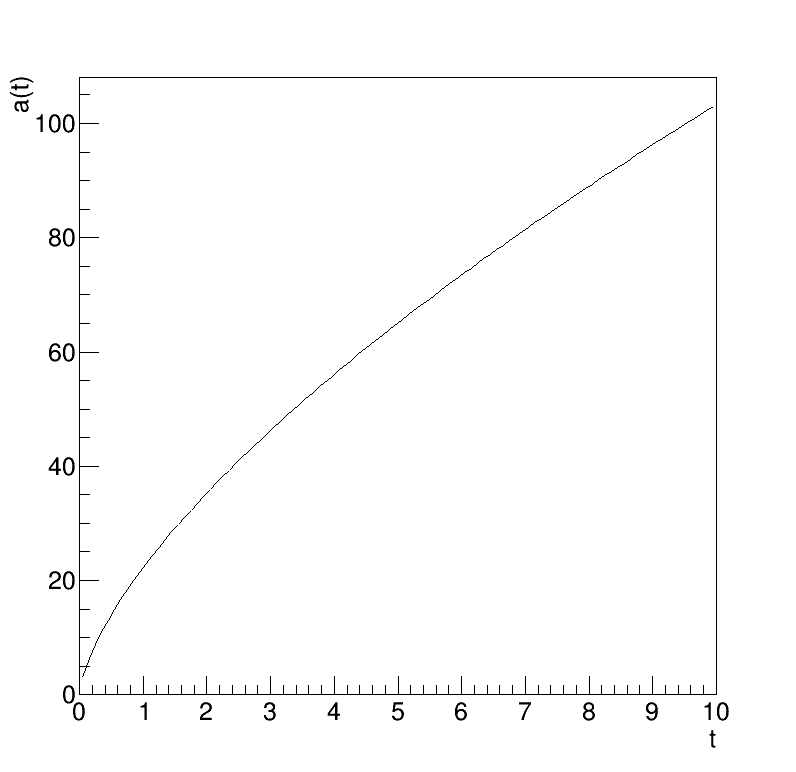
\includegraphics[width=0.4\textwidth]{ps1_plots/a_einstein}
\caption{The time evolution of the scale factor $a(t)$ in an Einstein-de Sitter Universe}
\end{figure}

% \section*{The Einstein-de Sitter Universe}
% %Find a way to cite http://www.nicadd.niu.edu/~bterzic/PHYS652/Lecture_05.pdf
% Here, $\Omega_{m,0}=1$ since the universe is matter dominated, and $k=0$ because the universe is flat.  The Friedmann equation thus reduces to
% \begin{equation}
% \left(\frac{\dot{a}}{a}\right)^2=\frac{8\pi G}{3}\rho
% \end{equation}
% Dodelson shows that conserved quantities in an expanding universe must follow
% \begin{equation}
% \frac{\partial \rho}{\partial t} + \frac{\dot{a}}{a}\left[3\rho+3P\right]=0
% \end{equation}
% In our case, $P$ can reasonably be set to zero.  Using the product rule, we can rearrange the above equation to
% \begin{equation}
% a^{-3}\left(\frac{\partial}{\partial t}\left[\rho a^3\right]\right)=0
% \end{equation}
% Since $\frac{\partial}{\partial t}\left[\rho a^{3}\right]=0$, this means that $\rho a^{3}=$ a constant.  We can thus claim that $\rho_m \propto a^{-3}$.

% Now, since $\Omega_{m,0}=1$, we know that $\rho_m=\rho_{cr}a^{-3}$.  The Friedmann equation now looks like
% $$\left(\frac{\dot{a}}{a}\right)^2=\frac{8\pi G}{3}\rho_{cr}a^{-3}$$
% Rearranging terms and splitting up the time derivative leaves us with
% $$\sqrt{a}\;da=\sqrt{\frac{8\pi G \rho_{cr}}{3}}\;dt$$
% Integrating both sides and using the fact that $a=0$ at the big bang, we get
% $$a^{\frac{3}{2}}=\frac{3}{2}\sqrt{\frac{8\pi G \rho_{cr}}{3}}\;t$$
% Multiplying through by $a^{\frac{2}{3}}$ and substituting in the definition of $\rho_{cr}=\frac{3H_{0}^{2}}{8\pi G}=9.21\cdot 10^{-27} kg/m^3$ we finally arrive at
% $$a(t)=\left(6\pi G\rho_{cr}\right)^{\frac{1}{3}}t^{\frac{2}{3}}$$
% \begin{figure}[h!]
% 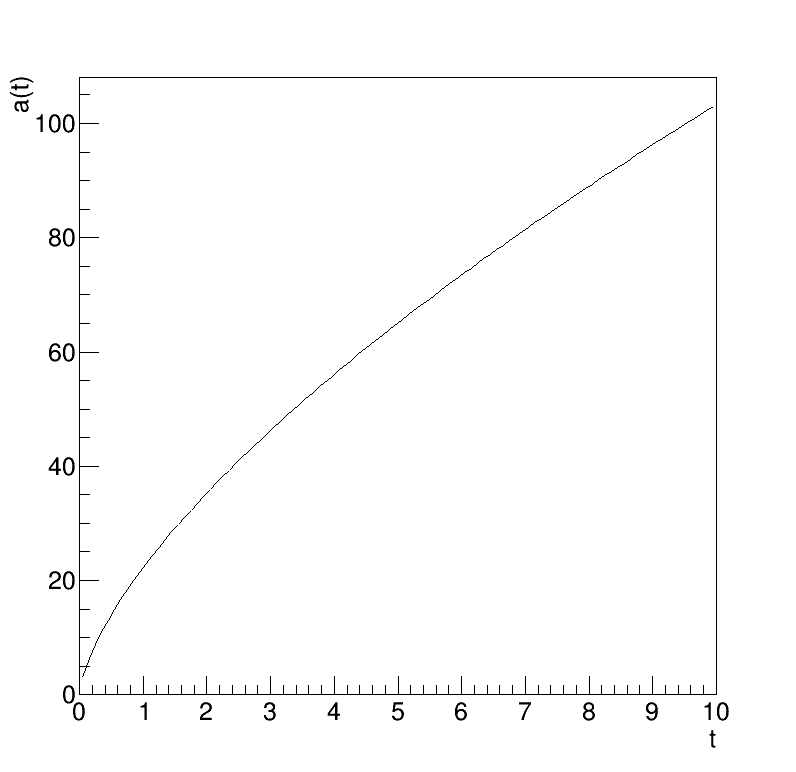
\includegraphics[width=0.5\textwidth]{ps1_plots/a_einstein}
% \caption{The time evolution of the scale factor $a$ in an Einstein-de Sitter Universe}
% \end{figure}

\bibliographystyle{unsrt}
\bibliography{ps1Sources}

%\begin{thebibliography}{99}
%
%\bibitem{wiki_scalefactor}
%Wikipedia contributors, "Scale factor (cosmology)," Wikipedia, The Free Encyclopedia, \url{http://en.wikipedia.org/w/index.php?title=Scale_factor_(cosmology)&oldid=642845167} (accessed February 11, 2015).
%
%\bibitem{carroll}
%Sean Carroll, Lecture Notes on General Relativity, \url{http://preposterousuniverse.com/grnotes/} (accessed February 11, 2015)
%
%\bibitem{scipy}
%Jones E, Oliphant E, Peterson P, et al. SciPy: Open Source Scientific Tools for Python, 2001-, \url{http://www.scipy.org/} 
%
%\bibitem{ROOT}
%Rene Brun and Fons Rademakers, ROOT - An Object Oriented Data Analysis Framework, Proceedings AIHENP'96 Workshop, Lausanne, Sep. 1996, Nucl. Inst. \& Meth. in Phys. Res. A 389 (1997) 81-86. See also \url{http://root.cern.ch/}.
%
%\end{thebibliography}

\end{document}